\section{Tipos de Dados e Variáveis}

\begin{frame}[fragile]
%[fragile, allowframebreaks=0.9]
 \frametitle{Tipos de Dados e Variáveis -- Introdução -- I}


\begin{itemize}

\item Em projetos de linguagens de programação há dois tipos 
verificação do tipo de dados: \underline{\textbf{estática}} e \underline{\textbf{dinâmica}}

  
  \pause 
  \item A verificação de tipos dados   \underline{estática} 
   em \textit{tempo de compilação}.
  
    \pause 
  \item Enquanto a \underline{dinâmica} em \textit{tempo de execução}.
  
  \pause 
  \item Linguagens fortemente tipadas, tais como C, Java e Pascal, 
  exigem que o tipo do dado (conteudo) seja do mesmo tipo da variável 
  ao qual este valor será atribuído. 
  Tudo isto é pré-definido durante a fase da \textit{compilação}.
  
  
\end{itemize}
\end{frame}


\begin{frame}[fragile]
%[fragile, allowframebreaks=0.9]
 \frametitle{Tipos de Dados e Variáveis -- Introdução -- II}
\begin{itemize}

  \item Nas linguagens interpretadas, com uma máquina virtual, 
  esta definição é feita durante a \textit{execução} do
  programa
  
  \pause 
  \item Prós e contras para o que é melhor, a discussão fica de lado neste momento
  
  \pause 
  \item Picat até o momento tem a tipagem \textbf{dinâmica}
  
\end{itemize}


\end{frame}


%%%%%%%%%%%%%%%%%%%%%%%%%%%%%%%%%%%%%%%%%%%%%%%%%%%%%%%%%%%%%%%%%%%%%

\subsection{Tipos de Dados}


\begin{frame}
	\frametitle{Tipos de Dados}
	

	\begin{figure}[!ht]
		\centering
		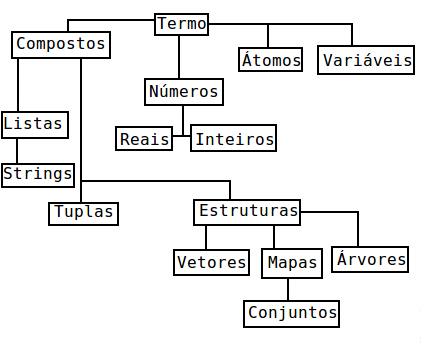
\includegraphics[width = .725\linewidth]{figures/tipos_dados_picat__traduzido3.png}
		\caption{Hierarquia dos Tipos de Dados}
		\label{fig:TiposDados}
	\end{figure}
	% imagem estilo da imagem de paradigmas
\end{frame}

%%%%%%%%%%%%%%%%%%%%%%%%%%%%%%%%%%%%%%%%%%%%%%%%%%%%%%%%%%%%%%%%%%%%%

\begin{frame}
%[fragile, allowframebreaks=0.9]
	\frametitle{Termos}

\begin{itemize}
	  \item Em Picat, variáveis e valores são \textit{genericamente} chamados de \textit{termos}
	
	  \pause 
	  \item Os valores são subdivididos em duas categorias, números e valores 
	compostos
	
		  \item Os números, por suas vez, podem ser inteiros ou reais, e valores compostos
	podem ser listas e estruturas
	
	%\pause 
	%\item Resumindo, em Picat tudo é \textit{termo}
	
	\end{itemize}	
\end{frame}

%%%%%%%%%%%%%%%%%%%%%%%%%%%%%%%%%%%%%%%%%%%%%%%%%%%%%%%%%%%%%%%%%%%%%

\begin{frame}[fragile]
	\frametitle{Átomos}
	
	\begin{itemize}
	  \item Átomos são constantes simbólicas, podendo ser delimitados ou não, por 
	aspas simples.
	
	\item Carácteres são representados por átomos de comprimento $1$.
	
	 	\item Átomos não delimitados por aspas simples, \underline{\textbf{nunca}} começam com uma letra maiúscula, nem número ou \textit{underscore}.

	\end{itemize} 

	  \pause 
	\begin{exampleblock}{Exemplos}
		\begin{verbatim}
		x   x_1   '_'   '\\'   'a\'b\n'   '_ab'   '$%'
		\end{verbatim}
	\end{exampleblock}
	
\end{frame}

%%%%%%%%%%%%%%%%%%%%%%%%%%%%%%%%%%%%%%%%%%%%%%%%%%%%%%%%%%%%%%%%%%%%%

\begin{frame}[fragile, allowframebreaks=0.9]

	\frametitle{Números}
	
	Números se dividem em:
	
	\begin{itemize}
		
		\item \textbf{Inteiro:} Inteiros podem ser representados por números binários, octais,
		decimais ou hexadecimais.
		% Dígitos em um número podem ser separados por um 
		% \textbf{underscore}, porém essa separação é ignorada pelo compilador.
		
	\end{itemize}
	
	\begin{exampleblock}{Exemplos}
		\begin{tabbing}
			aa \= aaa \= aaa \= aaa \= aaa \= aaa \= aaa \kill
			\> \texttt{12\_345} \> \> \> 12345 em notação decimal, usando \_ como separador \\
			\> \texttt{0b100} \> \> \> 4 em notação binária  \\
			\> \texttt{0o73} \> \> \>  59 em notação octal \\
			\> \texttt{0xf7} \> \> \>  247 em notação hexadecimal  
		\end{tabbing}
	\end{exampleblock}

\textcolor{red}{O \textbf{underscore} é ignorado pelo compilador e o interpretador.}

\framebreak
	
	\begin{itemize}
		
		\item \textbf{Real:} Números reais são compostos por um parte inteira, um ponto,
		 seguido por uma fração decimal, ou um expoente.
		
		\item Se existe uma parte inteira em um número real então ela deve ser seguida por uma
		fração ou um expoente. Isso é necessário para distinguir um número real de um número inteiro.
	\end{itemize}
	
	\begin{exampleblock}{Exemplos}
		\begin{verbatim}
		12.345   0.123   12-e10   0.12E10
		\end{verbatim}
	\end{exampleblock}
	
\end{frame}

%%%%%%%%%%%%%%%%%%%%%%%%%%%%%%%%%%%%%%%%%%%%%%%%%%%%%%%%%%%%%%%%%%%%%

\begin{frame}
	\frametitle{Compostos}
	\begin{itemize}
	  \item 	Termos compostos podem conter mais de um valor ao mesmo tempo. 
	  
	  \pause
    \item   Termos compostos são 
	acessados pela notação de índice, começando a partir de $1$ e indo até $N$, onde $N$
	 é o tamanho deste termo.

	  \pause
    \item 	Se dividem em \underline{Listas} e \underline{Estruturas}.
	
    
	\end{itemize}
	
	
	
\end{frame}

%%%%%%%%%%%%%%%%%%%%%%%%%%%%%%%%%%%%%%%%%%%%%%%%%%%%%%%%%%%%%%%%%%%%%

\begin{frame}
	\frametitle{Listas}
	
	Listas são agrupamentos de valores quaisquer sem ordem e sem tamanho pré-definido. Seu tamanho não é 
	armazenado na memória, sendo necessário recalcular sempre que necessário seu uso. Listas são 
	encapsuladas por colchetes.
	
	\begin{exampleblock}{Exemplos}
		[1,2,3,4,5] \: [a,b,32,1.5,aaac] \: ["string",14,22]
	\end{exampleblock}

\textcolor{red}{Há uma seção dedicada a esta poderosa  estrutura de dados!}
	
\end{frame}

%%%%%%%%%%%%%%%%%%%%%%%%%%%%%%%%%%%%%%%%%%%%%%%%%%%%%%%%%%%%%%%%%%%%%

\begin{frame}
	\frametitle{\textit{Strings} -- Lista de Carácteres}
	
	\textit{Strings} são listas especiais que contém somente carácteres. \textit{Strings} podem ser inicializadas como uma 
	sequência de carácteres encapsulados por aspas duplas, ou como uma sequência de carácteres dentro 
	colchetes separados por vírgulas.
	
	\begin{exampleblock}{Exemplos}
		"Hello" \: "World!" \: "\textbackslash n" \: [o,l,a,"\:",m,u,n,d,o] 
	\end{exampleblock}
	
\end{frame}

%%%%%%%%%%%%%%%%%%%%%%%%%%%%%%%%%%%%%%%%%%%%%%%%%%%%%%%%%%%%%%%%%%%%%

\begin{frame}
	\frametitle{Tuplas}
	\begin{itemize}
	  \item 	Tuplas é um conjunto de termos não-ordenados, podendo ser acessados por notação de índice assim como	listas.
	  
	  \item  Tuplas são estáticas, ou seja, os termos contidos em uma tupla não podem ser alterados, assim como	não podem ser adicionados ou removidos termos de tuplas.
	  
	\item   Tuplas são encapsuladas por parênteses e seus termos são separados por vírgulas.

	\end{itemize}
	
	\begin{exampleblock}{Exemplos}
		(1,2,3,4,5) \: (a,b,32,1.5,aaac) \: ("string",14,22)
	\end{exampleblock}
	
	\textcolor{red}{Em geral, usamos as tuplas dentro de listas.}
\end{frame}

%%%%%%%%%%%%%%%%%%%%%%%%%%%%%%%%%%%%%%%%%%%%%%%%%%%%%%%%%%%%%%%%%%%%%

\begin{frame}
	\frametitle{Estruturas (\textit{Functores})}
	
	Estruturas são termos especiais que podem ser definidos pelo usuário. Estruturas tomam a seguinte 
	forma: 
	
	\begin{displaymath}
	\texttt{{\$}s($t_1,\ldots,t_n$)}
	\end{displaymath}
	
	Onde \textit{`s'} é um átomo que denomina a estrutura, cada 
	\textit{`$t_i$'} é um de seus termos, e \textit{`n'} é a aridade ou tamanho da estrutura.
	
	\begin{exampleblock}{Exemplo}
		\$ponto(1,2) \: \$pessoa(jose, "123.456.789.00", "1.234.567")
	\end{exampleblock}
	
	\pause
	\textbf{\textcolor{red}{Temos 4 outras estruturas  que não usam o símbolo \$, são elas:}}
	
\end{frame}

%%%%%%%%%%%%%%%%%%%%%%%%%%%%%%%%%%%%%%%%%%%%%%%%%%%%%%%%%%%%%%%%%%%%%

\begin{frame}
	\frametitle{Vetores} [fragile, allowframebreaks=0.9]
	
	Vetores ou \textit{arrays} são estruturas especiais do tipo:
	\begin{center}
		 \texttt{\{$t_1$,$\ldots$,$t_{n}$\}}
		\end{center}
	
	\begin{itemize}
	 \pause
	   \item Vetor é um conjunto ordenado de tamanho $n$, delimitado por \texttt{'\{\}'}.
	   \item 	Vetores tem comportamentos análogo às listas, tanto é que quase todas as funções de listas
	são sobrecarregadas para vetores. 
	
		   \item A diferença entre vetores e listas é que vetores tem um tamanho  constante.
		   \item Vetores são muito práticos quando se manipula matrizes na entrada
		   
	 \end{itemize} 

	
	\begin{exampleblock}{Exemplos}
		\{1,2,3,4,5\} \: \{a,b,32,1.5,aaac\} \: \{"string",14,22\}
	\end{exampleblock}
	
\end{frame}

%%%%%%%%%%%%%%%%%%%%%%%%%%%%%%%%%%%%%%%%%%%%%%%%%%%%%%%%%%%%%%%%%%%%%

\begin{frame}
	\frametitle{Mapas, Conjuntos e \textit{Heaps}}
	
	\begin{itemize}
		\item \textbf{Mapas} são estruturas especiais que são conjuntos de relações do tipo \texttt{chave-valor}.
		
		\item \textbf{Conjuntos} são sub-tipos de mapas onde todos as chaves estão relacionadas com o átomo 
		\texttt{not\_a\_value}.
		
		\item \textit{Heaps} são árvores binárias completas representadas como vetores.
		Árvores podem ser do tipo \textit{máximo}, onde o maior valor está na raiz, ou \textit{mínimo}, 
		onde o menor valor esta na raiz.
	\end{itemize}
	
\end{frame}

%%%%%%%%%%%%%%%%%%%%%%%%%%%%%%%%%%%%%%%%%%%%%%%%%%%%%%%%%%%%%%%%%%%%%

\subsection{Variáveis}

\begin{frame}[allowframebreaks=0.90]
	\frametitle{Variáveis}
	
	\begin{itemize}
		
		\item Picat é uma linguagem de \underline{Tipagem Dinâmica}, ou seja, o tipo de uma variável 
		é validado durante a execução do programa
		
		
		\item Isto é, quando uma variável é criada, seu tipo não é instanciado
		
		\item Variáveis são análogas as da matemática, são símbolos que \textit{seguram} ou 
		representam um valor
		
		\item Ao contrário de variáveis em linguagens imperativas, variáveis em Picat não são
		endereços simbólicos de locais na memória
		
		\item Uma variável é dita \textit{livre} (\textit{free}) se não contém nenhum valor, e dita
		\textit{instanciada} (\textit{bound}) se ela contém um valor
		
		\item Uma vez que uma variável é instanciada, ela permanece com este valor na 
		execução atual
		
		\item Por isso, diz-se que variáveis em Picat são de \textit{atribuição única}
		
		\framebreak
		\item O nome de variáveis devem sempre ser iniciado com letras \textbf{\underline{maisculas}}
		ou  com o caráctere \textbf{\textit{underscore (\_)}}, porém;
		
		\begin{itemize}
			
			\item Variáveis cujo nome é unicamente um caractere \textbf{\_} são chamadas de 
			\textit{variáveis anônimas}.
			
			\item As 			\textit{variáveis anônimas} podem receber qualquer  valor
			 não os guardam  durante a execução do programa;
			
			\item Num mesmo programa, podem existir diversas variáveis anônimas, instanciadas durante a execução do mesmo
			
		\end{itemize}
		
	\end{itemize}
	
\end{frame}

%%%%%%%%%%%%%%%%%%%%%%%%%%%%%%%%%%%%%%%%%%%%%%%%%%%%%%%%%%%%%%%%%%%%%

\subsection{Unificação e Atribuição}

\begin{frame}
	\frametitle{Unficação e Atribuição}
	Há dois modos de definir valores a variáveis, a \underline{unificação}, que usa o operador 
	\textbf{=}, e a \underline{atribuição}, que usa o operador \textbf{:=}
\end{frame}

%%%%%%%%%%%%%%%%%%%%%%%%%%%%%%%%%%%%%%%%%%%%%%%%%%%%%%%%%%%%%%%%%%%%%

\begin{frame}[fragile]
	\frametitle{Unificação}
	% definição:
	% casamento de padrão
	% unificação (Algoritmo da Unificação)
	% montar uma figura talvez
	\begin{itemize}
		
		\item A \textbf{\underline{Unificação}} é uma operação que instância uma variável a um termo ou 
		padrão, substituindo toda a ocorrência dessa variável pelo valor a qual ela foi instanciada até que
		haja uma situação onde esta instanciação falhe, nesse momento a variável será reinstanciada e
		esse processo se repete.
		
		\item Caso ocorra uma instância que não falhe nenhuma situação a variável é unificada à este termo
		ou padrão.
		
		\item Uma instanciação é indefinida até que se encontre um valor que possa ser unificada a uma
		variável.
        
        \item Termos são ditos unificáveis se são idênticos ou podem ser tornados idênticos instanciado 
        variáveis nos termos.
		
	\end{itemize}
	
\end{frame}

%%%%%%%%%%%%%%%%%%%%%%%%%%%%%%%%%%%%%%%%%%%%%%%%%%%%%%%%%%%%%%%%%%%%%

\begin{frame}[fragile]
	
	\begin{exampleblock}{Exemplo}
		
		\begin{verbatim}
		Picat> X = 1
		X = 1
		Picat> $f(a,b) = $f(a,b)
		yes
		Picat> [H|T] = [a,b,c]
		H = a
		T = [b,c]
		Picat> $f(X,b) = $f(a,Y)
		X = a
		Y = b
		Picat> bind_vars({X,Y,Z},a)
		Picat> X = $f(X)
		\end{verbatim}
		
		A última consulta demonstra um caso do problema de ocorrência, onde o compilador de Picat não
		verifica se um termo ocorre dentro de um padrão. Isso cria um termo cíclico que não pode ser
		acessado. % Algo muito ruim
		
	\end{exampleblock}
	
\end{frame}

%%%%%%%%%%%%%%%%%%%%%%%%%%%%%%%%%%%%%%%%%%%%%%%%%%%%%%%%%%%%%%%%%%%%%
\begin{frame}[fragile]
	\frametitle{Atribuição}
	
	\begin{itemize}
		
		\item A \textbf{\underline{Atribuição}} é uma operação cujo intuito é simular a atribuição em
		linguagens imperativas, permitindo que variáveis sejam re-atribuídas valores durante a execução
		do programa
		
		\item Para isso, durante a compilação do programa, toda vez que a operação de unificação é 	
		encontrada, uma nova variável temporária será criada que irá substituir a variável que seria
		atribuída.
		
	\end{itemize}
	
\end{frame}

%%%%%%%%%%%%%%%%%%%%%%%%%%%%%%%%%%%%%%%%%%%%%%%%%%%%%%%%%%%%%%%%%%%%%

\begin{frame}[fragile]
	
	\begin{exampleblock}{Exemplo}
		
		\begin{verbatim}
		test => X = 0, X := X + 1,  X := X + 2, write(X).
		\end{verbatim}
		Neste exemplo $X$ é unificado a $0$, então, o compilador tenta unificar $X$ a $X+1$, porém $X$ já 
		foi unificado a um valor, portanto outras operações devem ser feitas para que esta atribuição seja
		possível.\\
		
		Nesse caso, o compilador irá criar uma variável temporária, $X1$ por exemplo, e à ela irá unir
		$X+1$, depois toda vez que $X$ for encontrado no programa o compilador irá substitui-lo por $X1$.\\
		
		O mesmo ocorre na atribuição $X1 := X1 + 2$, neste caso uma outra variável temporária será criada,
		$X2$ por exemplo, e o processo será repetido.\\
		
		Portanto, estas atribuições sucessivas são compiladas como:
		
		\begin{verbatim}
		test => X = 0, X1 = X + 1, X2 = X1 + 2, write(X2).
		\end{verbatim} 
		
	\end{exampleblock}
	
\end{frame}

%%%%%%%%%%%%%%%%%%%%%%%%%%%%%%%%%%%%%%%%%%%%%%%%%%%%%%%%%%%%%%%%%%%%%

\begin{frame}[fragile]
	
	\begin{exampleblock}{Exemplos de Variáveis Válidas}
		
		\begin{center}
			\begin{tabular}{|c|c|c|}\hline
				X1 & \textbf{\_} & \_ab \\ \hline
				X & A & Variavel \\ \hline
				\_invalido & \_correto & \_aa \\ \hline
			\end{tabular}
		\end{center}
		
		Relembrando, um nome de variável é válido se começa com letra maiúscula ou \_
		
	\end{exampleblock}
	
\end{frame}

%%%%%%%%%%%%%%%%%%%%%%%%%%%%%%%%%%%%%%%%%%%%%%%%%%%%%%%%%%%%%%%%%%%%%

\begin{frame}[fragile]
	
	\begin{exampleblock}{Exemplos de Variáveis Inválidas}
		
		\begin{center}
			\begin{tabular}{|c|c|c|}\hline
				\verb!1_Var! & variavel & valida\\ \hline
				$23$ & \verb!"correto! & \verb!'termo!\\ \hline
				\verb+!numero+ & \verb!$valor! & \verb!#comum!\\ \hline
			\end{tabular}
		\end{center}
		
		Relembrando, um nome de variável é inválido se começa com números ou símbolos que não sejam 
		\_ ou letra minúscula
		
	\end{exampleblock}
	
\end{frame}

%%%%%%%%%%%%%%%%%%%%%%%%%%%%%%%%%%%%%%%%%%%%%%%%%%%%%%%%%%%%%%%%%%%%%

\subsection{Tabela de Operadores} 
\begin{frame}[fragile]
	
	\begin{table}
		\caption{\label{Operadores Aritméticos}Operadores Aritméticos em Ordem de Precedência}
		\begin{center}
			\begin{tabular}{ c|c } \hline
				\texttt{$X$ ** $Y$}  &  Potenciação \\ \hline 
				\texttt{$X$ * $Y$} &    Multiplicação \\ \hline 
				\texttt{$X$ / $Y$} &    Divisão, resulta em um real \\ \hline 
				\texttt{$X$ // $Y$} &    Divisão de Inteiros, resulta em um inteiro \\ \hline 
				\texttt{$X$ mod $Y$} &   Resto da Divisão\\ \hline
				\texttt{$X$ + $Y$} & Adição \\ \hline 
				\texttt{$X$ - $Y$} &   Subtração \\ \hline 
				{\tt $Inicio$ \verb!..! $Passo$ \verb!..! $Fim$} & Uma série (lista) de números com um passo\\ 
				\hline 
				{\tt $Inicio$ \verb!..! $Fim$}  &   Uma série (lista) de números com passo 1 \\ \hline
			\end{tabular}
		\end{center}
	\end{table}
	
\end{frame}

%%%%%%%%%%%%%%%%%%%%%%%%%%%%%%%%%%%%%%%%%%%%%%%%%%%%%%%%%%%%%%%%%%%%%

\begin{frame}[fragile]
	\begin{table}
		\caption{Tabela de Operadores Completa em Ordem de Precedência}
		\begin{center}
			\begin{tabular}{ c|c } \hline
				Operadores Aritméticos & Ver Tabela \ref{Operadores Aritméticos}\\ \hline
				\verb-++-  & Concatenação de Listas/Vetores \\ \hline 
				\verb+=+  \verb+:=+  & Unificação e Atribuição\\ \hline
				\verb+==+ \verb+=:=+ & Equivalência e Equivalência Numérica\\ \hline
				\verb+!=+ \verb+!==+ & Não Unificável e Diferença\\ \hline
				\verb+<+  \verb+=<+ \verb+<=+ & Menor que\\ \hline
				\verb+>+  \verb+>=+ & Maior que\\ \hline
				\verb+in+ & Contido em\\ \hline
				\verb+not+ & Negação Lógica \\ \hline 
				\verb+,+  $\&\&$ & Conjunção Lógica \\ \hline 
				\verb+;+  $|$$|$ & Disjunção Lógica \\ \hline 
			\end{tabular}
		\end{center}
	\end{table}
\end{frame}

%%%%%%%%%%%%%%%%%%%%%%%%%%%%%%%%%%%%%%%%%%%%%%%%%%%%%%%%%%%%%%%%%%%%%

\subsubsection{Operadores Especiais}

\begin{frame}[fragile,c]
    \frametitle{Operadores Especiais \textrm{\MakeUppercase{\romannumeral 1}}}
    
    \begin{block}{Operadores de Termos Não Compostos}

		\begin{enumerate}
    
            \item \textbf{Equivalência}(\verb+==+): Compara se dois termos são iguais.\\No caso de termos
            compostos, eles são ditos equivalentes se todos os termos contidos em si são equivalentes. O 
            compilador considera termos de tipos diferentes como totalmente diferentes, portanto a comparação 
            $1.0 == 1$ seria avaliada como falsa, mesmo que os valores sejam iguais. Nesses casos, usa-se a 
            \emph{Equivalência Numérica}.

            \item \textbf{Equivalência Numérica}(\verb+=:=+): Compara se dois números são o mesmo valor.
            Não deve ser usada com termos que não são números.

            \item \textbf{Diferença}(\verb+!==+): Compara se dois termos são diferentes.\\Mesmo que a negação da 
            equivalência.

            \item \textbf{Não Unificável}(\verb+!=+): Verifica se dois termos não são unificáveis. Termos são 
            ditos unificáveis se são idênticos ou podem ser tornados idênticos instanciando variáveis destes 
            termos.
    	\end{enumerate}
    \end{block}
    
\end{frame}

%%%%%%%%%%%%%%%%%%%%%%%%%%%%%%%%%%%%%%%%%%%%%%%%%%%%%%%%%%%%%%%%%%%%%

\begin{frame}

	\begin{exampleblock}{Exemplos}
    	
    	\begin{enumerate}
    	
          \item $a\:$==$\:a$, \: $[1,2,3]\:$==$\:[1,2,3]$, \: $Var1\:$==$\:Var2$\\
          \pause
          $yes$, $yes$, Depende dos Valores (padrão $no$)
          \medskip
          \pause
          
          \item $1.0\:$==$\:1$\\
          \pause
          $no$
          \medskip
          \pause
          
          \item $1.0\:$=:=$\:1$, \: $1.2\:$=:=$\:1$\\
          \pause
          $yes$, $no$
          \medskip
          \pause

          \item $1.0\:$!==$\:1$, \: $Var3\:$!==$\:Var4$\\
          \pause
          $yes$, Depende dos Valores (padrão $yes$)
          \medskip
          \pause

          \item $1.0\:$!=$\:1$, \: aa\:$!=$\:bb, \: $Var1\:$!=$\:Var5$\\
          \pause
          $yes$, $yes$, $no$
          
        \end{enumerate}
	\end{exampleblock}
    
\end{frame}

%%%%%%%%%%%%%%%%%%%%%%%%%%%%%%%%%%%%%%%%%%%%%%%%%%%%%%%%%%%%%%%%%%%%%

\begin{frame}[fragile,c]
    \frametitle{Operadores Especiais \textrm{\MakeUppercase{\romannumeral 2}}}
    
    \begin{block}{Operadores de Termos Compostos}
    	
    	\begin{enumerate}
        
            \item \textbf{Concatenação}\/ (\verb!++!): concatena duas listas ou vetores, tornando o primeiro termo 
            da segunda lista no termo seguinte ao último termo da primeira lista.

            \item \textbf{Separador}\/ (\verb!H | T!): separa uma lista \emph{L} em seu primeiro termo \emph{H}, 
            chamado de cabeça (em inglês \textit{Head}), e o resto da lista \emph{T}, chamado de cauda (em inglês \textit{Tail}).

            \item \textbf{Iterador}\/ (\verb!X in L!): itera pelo termo composto \emph{L}, instanciando um termo
            não composto \emph{X} aos termos contidos em \emph{L}. Bastante utilizado para iterar por listas.
	%iterador
            \item \textbf{Sequência }\/ (\verb!Inicio..Passo..Fim!): Gera uma lista ou vetor, começando 
            (inclusivamente) em \textit{Inicio} incrementando por \textit{Passo} e parando (inclusivamente) em 
            \textit{Fim}. Se \textit{Passo} for omitido, é automaticamente atribuído 1. Se usado dentro do 
            índice de uma lista ou vetor resultará na porção da lista dentro deste intervalo.
            
    	\end{enumerate}
        
    \end{block}
    
\end{frame}

%%%%%%%%%%%%%%%%%%%%%%%%%%%%%%%%%%%%%%%%%%%%%%%%%%%%%%%%%%%%%%%%%%%%%

\begin{frame}
	
    \begin{exampleblock}{Exemplos}
		
        \begin{enumerate}
        
			\item $[1,2,3]$\:$++$\:$[4,5,6]$, \: $[]$\:$++$\:$[1,2,3]$, \: $[]$\:$++$\:$[]$\\
            \pause
            $[1,2,3,4,5,6]$, \:$[1,2,3]$, \:$[]$
            \medskip
            \pause
            
            \item $L = [1,2,3]$,\:\:$[H|T] = L$\\
            \pause
            $L = [1,2,3]$\\ \pause
            $H = 1$\\ \pause
            $T = [2,3]$
            \medskip
            \pause
            
            \item $foreach(X\:in\:[1,2,3])$\:\:$printf("\%w\:",X)$\:\:$end$\\
            \pause
            $1$ $2$ $3$
            \medskip
            \pause
            
            \item $X\:=\:1..10$,\:\:$Y\:=\:0..2..20$,\:\:$Z\:=\:10..-1..1$\\
            \pause
            $X = [1,2,3,4,5,6,7,8,9,10]$\\ \pause
            $Y = [0,2,4,6,8,10,12,14,16,18,20]$\\ \pause
            $Z = [10,9,8,7,6,5,4,3,2,1]$
            
		\end{enumerate}
        
	\end{exampleblock}
    
\end{frame}
